\documentclass[titlepage, a4paper,10pt]{article}
\usepackage[english]{babel}
\usepackage[utf8x]{inputenc}
\usepackage{listings}
\usepackage{graphicx}
\usepackage[dvips]{hyperref}
\hypersetup{bookmarks = true}
\hypersetup{pdftitle = MetaDoc Client Documentation}
\hypersetup{pdfauthor = Bjørnar Grip Fjær}
\hypersetup{pdfsubject = MetaDoc Client Documentation}
\hypersetup{colorlinks = true}
\hypersetup{urlcolor = black}
\hypersetup{linkcolor = black}
\hypersetup{citecolor = black}
\hypersetup{filecolor = black}
\hypersetup{linktocpage = true}
\addtolength{\oddsidemargin}{0.85cm}
\addtolength{\evensidemargin}{-1.5cm}
\addtolength{\textwidth}{0.75cm}
%\addtolength{\topmargin}{-1.0cm}
\addtolength{\textheight}{1cm}
\newcounter{scriptcounter}
\setcounter{scriptcounter}{1}
\newcommand\rawcode[3]{{#1 \lstinputlisting[label=#2]{#3}}}
\newcommand\scriptcode[4][script\arabic{scriptcounter}]{
        \lstset{language=#4,
                emph={asmlinkage, \_\_user, ENTRY, foreach, \_\_init, \_\_exit},
                numbersep=15pt,
                numbers=left,
                numberstyle=\scriptsize,
                frame=tb,
                tabsize=8,
                commentstyle=\texttt,
                keywordstyle=\bfseries,
                emphstyle=\bfseries,
                linewidth=\textwidth,
                showstringspaces=false
                frame=shadowbox,
                rulesepcolor=\color{blue},
                caption=#2}
        \rawcode{\scriptsize}{#1}{#3}
        \addtocounter{scriptcounter}{1}}

\newcommand\inlinecode[1]{{ \texttt{\small #1} }}

% Note that for glossary list to work, `makeglossaries doc` must be run
\usepackage{glossaries}
\makeglossaries
\newacronym{hpc}{HPC}{High Performance Computing}
\newacronym{xml}{XML}{Extensible Markup Language}
\newacronym{mapi}{MAPI}{MetaDoc API}
\newacronym{dtd}{DTD}{Document Type Definition}
\newacronym{api}{API}{Application programming interface}
\newacronym{http}{HTTP}{Hypertext Transfer Protocol}
\newacronym{ssl}{SSL}{Secure Socket Layer}
\newacronym{tls}{TLS}{Transport Layer Security}

\title{MetaDoc Client Documentation\\\small{Version 0.1.0}}
\author{Bjørnar Grip Fjær}
\date{\today}

\begin{document}
\maketitle

\pagenumbering{roman}
\tableofcontents
\newpage

\pagenumbering{arabic}
\newpage
\section{Introduction}
MetaDoc is created as a way to securely transport data between a server and 
sites. It is created to improve the flow of information between \gls{hpc} sites
and Uninett Sigma \cite{improvingflow}.

MetaDoc consists of a client, running at the site, and a server running at the
Metacenter. MetaDoc takes care of authenticating the client on the server,
packing and unpacking the data to and from \gls{xml}, and transporting the data
securely between client and server. 

If you wish to get the client up and running as quickly as possible, the
MetaDoc Client Quick Start Guide is a good place to start
\cite{quick_start_guide}.

\begin{figure}[h!]
    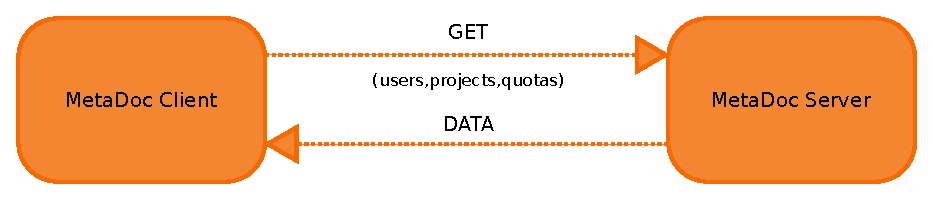
\includegraphics[width=\textwidth]{img/get_data}
    \caption{Client requesting data from server}
    \label{fig:get_data}
\end{figure}

Figure \ref{fig:get_data} shows how the client requests data from the server.
The MetaDoc client provides the interface for retrieving this data, and it is
then up to the site to decide how to handle the recieved data. 

\begin{figure}[h!]
    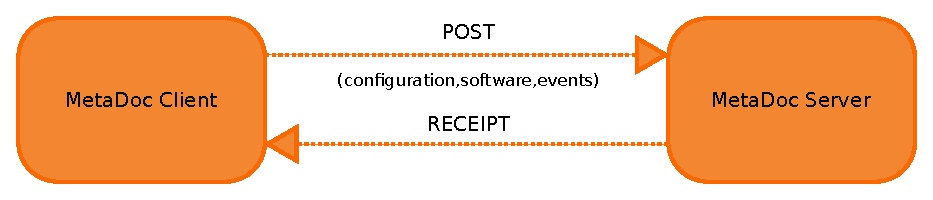
\includegraphics[width=\textwidth]{img/post_data}
    \caption{Client sending data to server. Server returns a receipt for
    recieved data.}
    \label{fig:post_data}
\end{figure}

In figure \ref{fig:post_data}, data is sent from the client to the server. On
recieving the data, the server will return a receipt, telling the client that
the data has been processed and accepted or rejected. 

In section \ref{sec:overview}, an overview of the MetaDoc client is given. It
explains what is done by the standard client, and how the client can run. 

Section \ref{sec:client_api} explains how to customize the MetaDoc client in
order to process the data sent between the client and server. 

Section \ref{sec:server_api} goes through the server side API. It explains how
the server acts in response to requests by the MetaDoc client. 

The \gls{xml} document used to send data between the client and server is
explained in section \ref{sec:xmldoc}. 

Section \ref{sec:useful_classes} describes some useful classes and modules
provided by the MetaDoc client for use when extending the client to send or
recieve more data. 

A guide to extending the client is given in section \ref{sec:extending}. This
is a step for step guide that explains what is needed in order for the client
to send or recieve more data. 

The information flow between client and server is explained in more detail in
section \ref{sec:information_flow}.

An explanation of possible errors that may occour during usage of the MetaDoc
client is given in section \ref{sec:errors}. 


\newpage
\section{Overview}
\label{sec:overview}
Usage of the MetaDoc client is done mainly through the use of \texttt{mapi.py}.
\texttt{mapi.py} takes care of sending and retrieving data to and from the
server, caching any data that could not be sent, and validating \gls{xml} data
received.

\subsection{Configuration}
\label{sec:metadoc_conf}
The MetaDoc client uses a configuration file \texttt{metadoc.conf}. This file
\textit{must} be placed in the same folder as the client itself. Listing
\ref{lst:config} provides an example of a basic configuration file.

The configuration is in INI format and defines a section named
\texttt{MetaDoc}.

\paragraph{Required parameters:}

\begin{description}
    \item[host] \textbf{baseurl} for the MetaDoc Server that the client should
        communicate with.
    \item[key]  Absolute path to the clients X.509 certificate key file. This
        should be the private key for \textbf{cert}, and is used to encrypt
        data passed to the server.
    \item[cert] Absolute path to the clients X.509 certificate file. This is used
        to authenticate the client with the server. See section
        \ref{sec:authentication} for more information.
    \item[site\_name]   The name of the site the client is running on. 
    \item[ca\_certs]    Absolute path to a file containing certificates for the
        CA that signs the MetaDoc server's certificate.
\end{description}

\paragraph{Optional parameters:}

\begin{description}
    \item[trailing\_slash]  Whether the client should append a trailing slash
        at the end of URLs used to connect to the server. At the moment, this
        should be set to \texttt{True}.
    \item[valid]    Initially set to \texttt{False} when \texttt{mapi.py}
        creates a sample configuration file. This is set to avoid running the
        client without being properly configured. If this value is present, it
        \textit{must} be set to \texttt{True} or \texttt{yes}.
\end{description}

\texttt{mapi.py} will create a initial configuration file if one is missing
when it starts. This can be used as the basis for a configuration file. 

\scriptcode[lst:config]{Example of a basic configuration file}{examples/configuration/metadoc.conf}{}

\subsection{Handles}
\label{sec:handles}
A handle is an option passed to the client when running the script.

\texttt{mapi.py} takes handles that tell the script what information to send
or retrieve to or from the server. All handles can be mixed together
\textit{except} for handles that override each other. Handles that overrides
others are explicitly stated below.

\texttt{mapi.py} takes the following handles:

\begin{description}
    \item[-h, --help]   Displays a short help message explaining the handles
    that may be passed to \texttt{mapi.py}. Overrides any other handles.
    \item[-v, --verbose]    Verbose mode. Prints information about progress and
    information sent and received between client and server. 
    \item[-q, --quiet]  Quiet mode. Prints nothing unless the program fails.
    Overrides \textbf{-v}, \textbf{--verbose}.
    \item[-l \textless log level\textgreater, --log-level=\textless log
    level\textgreater] Sets the log level for the program. See section 
    \ref{sec:logging} for more information about what is logged at different 
    levels.
    \item[-n, --no-cache]   Prevents the client from sending any cached data.
    If any errors occour when the client runs with this handle, data from this
    run will \textit{not} be cached. For more information about caching, see
    section \ref{sec:caching}.
    \item[-e]   Sends event data from client to server.
    \item[-c]   Sends configuration data from client to server.
    \item[-s]   Sends software data from client to server.
    \item[-u]   Retrieves user data from the server.
    \item[-a]   Retrieves allocation data from server.
    \item[-p]   Retrieves project data from server.
    \item[--dry-run]    Does a dry run, not sending any data to server. Does
        not retrieve cached data, and does not save any data to cache.
        Should be run with verbose to see data that would be sent.
    \item[--all]    Sends and retrieves all possible data. Equal to -ecsuap.
    \item[--send-all]   Sends all possible data. Equal to -ecs.
    \item[--fetch-all]  Retrieves all possible data. Equal to -uap.
\end{description}

\subsection{Logging}
\label{sec:logging}
The client logs data to \texttt{/var/log/mapi/}. The folder must be readable
and writable for the user that runs the.  The client creates a new log file
each day it runs, with the naming schema:
\texttt{metadoc.client.YYYY-mm-dd.log}. 

The client has five different logging levels. The list below gives an overview
of what is logged at the different levels. The higher items in the list contain
everything below as well, so that with a log level set to \textbf{error} will
also contain \textbf{critical} logging.

The log level defaults to \textbf{warning} if no log level set on execution.

\begin{description}
    \item[debug]    Debugging information, used for development and error
    checking.
    \item[info] Information about what is happening during execution, such as
    items sent or received to/from the server.
    \item[warning]  Warnings occurring during execution, mainly problems that
    will not cause a failure but that should be addressed.
    \item[error]    Errors that cause partial failure of the execution, such as
    being unable to connect to the server.
    \item[critical] Critical failures that causes the execution to halt, or
    errors in the program code itself.
\end{description}

\subsection{Caching}
\label{sec:caching}
The client caches data to \texttt{/var/cache/mapi/}. Files are named after the
data type that is cached in each file. The user running the client must have
read and write access to this folder. 

The client will cache any information that is not accepted by the server, 
\textit{unless} the server returns a receipt for the information that marks the 
information as invalid or malformed in some way, such that the information will 
not be accepted if resent at a later date. See section \ref{sec:errors} for
more information about errors.

Data the client sends may be marked so that it will not resend any cached data
when the client is run with the same handle. This is mainly for use for full
updates, such as software and configuration, where any cached data would be
outdated or duplicates if sent together with a new run.

If the \textbf{-n} or \textbf{--no-cache} handles are passed, the script will
ignore any cached data completely and run as if it didn't exist. The client
will also \textit{not} cache any data on this run. The cached data will then be
processed on the next run where \textbf{-n} or \textbf{--no-cache} is not
passed. 


\newpage
\section{MetaDoc Client API}
\label{sec:client_api}

The MetaDoc client calls a specified function based on the data passed between
client and server. Only one type of data should be sent per document, and both
the client and the server only checks for the expected type of data in the
recieved \gls{xml} document. 

Each data type has a named container element within the \gls{xml} document,
which there should only be one of per document. If a list of data is passed
between server and client, the list should be placed inside a container
element. The name of the container element is used in naming modules and
classes in order to ease readability of code. 

An example of such a container is \texttt{users}, which holds
\texttt{user\_entry} elements. An example of a MetaDoc \gls{xml} document with
a list of users is shown in listing \ref{lst:userlistexample}.

\scriptcode[lst:userlistexample]{User list XML example}{examples/xml/container.xml}{XML}

The naming of the class that handles the data passed between server and client
on the client side depends on whether data is passed from client to server, or
the other way around. 

\subsection{Sending data}
\label{sec:customizing_client_send}
Before data can be sent, the \gls{xml} document must be assembled. Because
there is not always a standard way to populate this data on every site, a
custom class is created. This class should be found under
\texttt{custom.site<name>.Site<Name>}, where \texttt{<name>} is the name of the
container element in the \gls{xml}, and \texttt{<Name>} is the name capitalized
(e.g.  \texttt{config} would use \texttt{custom.siteconfig.SiteConfig}). This
class should inherit from \\ \texttt{custom.abstract.MetaOutput}. 

When the client is ready to fetch these items, the function \texttt{populate()}
in this class is called. This function will gather the information to send,
creating elements found in
\texttt{<name>.definition.<Name>.legal\_element\_types} for this information
and placing these items in \texttt{self.items}. 

An example of such a class for the imaginary \texttt{posts} data is shown
below.

\scriptcode{custom.siteposts}{examples/metaelements/custom/siteposts.py}{python}

The client will then take care of packing data to \gls{xml}, sending the data
to the server, processing the receipt returned from the server and caching any
data that was not accepted by the server. For more information on caching, see
section \ref{sec:caching}.

\subsection{Recieving data}
\label{sec:customizing_client_recieve}
The client will take care of fetching the data from the server, unpacking the
\gls{xml} and creating objects based on the type of data recieved. Once this is
done, a function called \texttt{process()} will be called on the class
\texttt{custom.update<name>.Update<Name>}. When this function is called, the
object's \texttt{self.items} should be a list of \\
\texttt{<name>.definition.<Name>} objects.

Examples for producing files similar to the ones now in use based on
information transferred through MetaDoc is given in
\texttt{doc/examples/custom/}.

\subsection{Summary}
\texttt{process()} and \texttt{populate()} are the key functions that are used
to customize how the client handles data passed between the MetaDoc client and
server. 


\newpage
\section{MetaDoc Server API}
\label{sec:server_api}

The MetaDoc server implements a REST-like \gls{api} \cite{rest}, however, there
are certain differences from REST noted in section \ref{sec:diff_from_rest}.

When the client performs a GET request on an available URL, the server should
return an \gls{xml} document, or a \gls{http} status code referring to an
error.  The \gls{xml} document should follow the MetaDoc \gls{dtd}
\cite{metadoc_dtd}. Each URL only returns data from the requested data type.
This means that a request to \textbf{/allocations/} will return a MetaDoc
\gls{xml} document containing only an \texttt{<allocations>} directly on the
\texttt{<MetaDoc>} root, with \texttt{<all\_entry>} tags as children of
\texttt{<allocations>}.  The client should disregard any information outside
\texttt{<allocations>} when connecting to \textbf{/allocations/}. 

In order to send data to the server, the client performs a POST request, with
the POST data variable \texttt{metadoc} containing a MetaDoc \gls{xml}
document. The server will only accept data from the data type specified in the
URL, and will disregard any other information. This means that a POST to
\textbf{/events/} should be a MetaDoc \gls{xml} document containing a
\texttt{<events>} tag directly on the \texttt{<MetaDoc>} root, with any number
of \texttt{<resourceUp>} and \texttt{<resourceDown>} tags as children of
\texttt{<events>}. 

When this data is sent to the server, the server should return a MetaDoc
\gls{xml} document containing a \texttt{<receipts>} tag, with a
\texttt{<r\_entry>} tag for each element received that has an
\textbf{id}-attribute. This allows for a very fine grained error reporting.

\subsection{Available URLs}

\begin{description}
    \item[/allocations/] Retrieves a list of allocations/quotas relevant
        to the client
    \item[/users/] Retrieves a list of users for the client
    \item[/projects/] Retrieves a list of projects relevant to the
        client
    \item[/config/] Sends system configuration to server
    \item[/events/] Sends site events to the server
    \item[/software/] Sends system software to server
\end{description}

\subsection{Authentication}
\label{sec:authentication}
The server uses X.509 certificates to authenticate the client. In order for the
site to be authenticated properly, the server must be aware of the client's
certificate prior to the request, and the correct owner of the certificate must
be saved on the server. This \textit{must} be the same as the value for
\texttt{site\_name} set in the MetaDoc configuration (see section
\ref{sec:metadoc_conf}).

\subsection{Differences from REST}
\label{sec:diff_from_rest}

There are certain differences in the \gls{api} compared to the REST
specification. The MetaDoc Server \gls{api} makes use of \gls{http} POST where
\gls{http} PUT should be used in accordance with REST. This is due to
limitations in standard Python libraries.

Because the MetaDoc Server does not give the client access to delete or replace
data on the server, replacing PUT with POST will not cause problems.

\subsection{Server HTTP responses}

The server makes use of \gls{http} status codes to identify what error has
occurred if the server is unable or unwilling to process the request from the
server.  Table \ref{tbl:http_status_codes} contains a list of status codes the
server returns, and why these status codes occur. 

Any return code except for 200 is considered to be an error.

\begin{table}[h!]
    \centering
    \caption{List of HTTP status codes used by the MetaDoc Server}
    \begin{tabular}{|l|l|p{7cm}|}
        \hline
        \textbf{Code} & \textbf{Official name} & \textbf{\gls{mapi}-reason} \\
        \hline
        200 & 200 OK & The server has processed the request and should return
        an \gls{xml} document. \\
        \hline
        400 & 400 Bad Data & The data excepted from the client was not sent, or
        the \gls{xml} document did not validate against the \gls{dtd} or was
        malformed \gls{xml}. \\
        \hline
        403 & 403 Forbidden & The client certificate was not recognized as an
        authorative source for the site given in the \gls{xml} document. \\
        \hline
        404 & 404 Not found & The URL the client is attempting to access is not
        available on the server. Check host in \texttt{metadoc.conf}. If host
        is correct, make sure client and server uses same version. See section
        \ref{sec:version} for more information on version differences. \\ 
        \hline
        500 & 500 Server Error & The server failed to process the request. This
        does not include errors that return a receipt. \\
        \hline
        501 & 501 Not Implemented & The request method is not implemented for
        this URL. This will happen if the client attempts to use a request
        method that is not implemented for this URL, such as using the POST
        request method against an URL that only supports GET. \\
        \hline
    \end{tabular}
    \label{tbl:http_status_codes}
\end{table}


\newpage
\section{XML document}
\label{sec:xmldoc}
The XML document should follow the form described in the MetaDoc DTD 
\cite{metadoc_dtd}. Below certain conventions used in the XML build is 
explained. Any alterations to the DTD should follow these conventions in order
for the client and server to continue functioning normally. 

\subsection{Document build}
Any type of information sent should only create one direct child of the root
element, \texttt{<MetaDoc>}. This means that when lists of information is sent, 
the list elements should be placed within a container element, and \textit{not} 
directly in the root element. The container element should have an self
explanatory name about the information passed. 

An example is that \texttt{<user\_entry>} elements are placed within a
\texttt{<users>} element. Here \texttt{<users>} is considered the container
element, and there should only be one of them in each MetaDoc XML document.
\texttt{<users>} may contain any number of \texttt{<user\_entry>} elements. 

\subsection{Dates}
All dates in the document should be on the form specified by RFC3339 
\cite{rfc3339}. The \texttt{utils} module provides a function 
\texttt{date\_to\_rfc3339} that takes a \texttt{datetime.datetime} object and 
returns a string on RFC3339 form. It also provides a function
\texttt{rfc3330\_to\_date} which will return a \texttt{datetime.datetime}
object from a proper RFC3339 string, or \textbf{False} if the string is not a
correct RFC3339 date.

\subsection{Special attributes}
The \textbf{id} attribute of elements have a special function in MetaDoc. This 
attribute is used to identify the object when recieving receipts from the server 
whether elements have been added. The attribute is \textit{not} saved in caching 
to avoid duplicate \textbf{id}s when resending cached data together with new 
data. If you want to give elements a special identifier that should be saved, it 
must be called something other than \textbf{id}.


\newpage
\section{Useful classes and modules}
\label{sec:useful_classes}
The MetaDoc client defines a series of classes and modules that are used to
define the \gls{xml} data passed between client and server. 

\texttt{MetaElement} refers to \texttt{metaelement.MetaElement}, and
\texttt{MetaDoc} refers to \\ \texttt{metadoc.MetaDoc}.

\subsection{MetaDoc}
The class \texttt{MetaDoc} is used to define the document itself. It provides
functionality to alter the document structure, find elements within the
document and generate \gls{xml} data from the document. It contains a series of
\texttt{MetaElement} sub classes that defines the content within the document.

\subsection{MetaElement}
\texttt{MetaElement} is used to define content within the document.  The class
is ment to be a parent class for other classes that defines particular
elements. An element is equal to an \gls{xml} tag, such as \texttt{<users>} or
\texttt{<resourceUp>} in a MetaDoc \gls{xml} document. An instance of such a
sub class is used to define a particular tag in the \gls{xml} document, with
attributes and content.  

\subsubsection{Class variables}

\paragraph{xml\_tag\_name}
Each \texttt{MetaElement} sub class should define a class variable \\
\textbf{xml\_tag\_name}, that should be a string containing the name of the
\gls{xml} tag the class describes. For the sub class defining the
\texttt{<users>} tag, this should be set to ``users``. 

\paragraph{url}
A \texttt{MetaElement} sub class that defines a main container element, that
is, an element that is placed as a direct child of the root node
\texttt{<MetaDoc>} in the \gls{xml} document, should also define a class
variable \textbf{url} that is a string containing the particular part of the
URL that is used to send or retrieve information for the data type passed. If
the type of data is a list of users, and it should retrieve the list of users
from the url \textbf{/users/}, the \textbf{url} class variable should be set to
``users``.

The classes that define a main container element should also define either the
class variable \textbf{update\_handler} or \textbf{site\_handler}, depending on
whether the data is ment to be recieved from the server or sent from the
client, respectively. 

\paragraph{update\_handler}
\textbf{update\_handler} should be a sub class of \\
\texttt{custom.abstract.MetaInput}. This class should be placed in \\
\texttt{custom.update<name>.Update<Name>}, so for users this would be \\
\texttt{custom.updateusers.UpdateUsers}. When data of the type defined by the
\texttt{MetaElement} sub class is recieved, an instance of
\textbf{update\_handler} will be created, and the instance's
\textbf{self.items} will be populated with a list of \texttt{MetaElement} sub
classes. Then the \textbf{update\_handler}'s \texttt{process()} function will
be called.  Normally, \textbf{self.items} should be of length 1.

\paragraph{site\_handler}
\textbf{site\_handler} should be a sub class of
\texttt{custom.abstract.MetaOutput}. This class should be placed in
\texttt{custom.site<name>.Site<Name>}, so for events this would be
\texttt{custom.siteevents.SiteEvents}. When the script is called to send data
of the type defined by the \texttt{MetaElement} sub class, an instance of
\textbf{site\_handler} is created, and the instance's \texttt{populate()}
function is called. \texttt{populate()} should populate the instance's
\textbf{self.items} with a list of \texttt{MetaElement} sub classes. When
\texttt{populate()} is done, \textbf{self.items} is added to the
\texttt{MetaElement} sub class instance's \textbf{self.sub\_elements}.

\subsubsection{Allowed sub\_elements}
There are certain restrictions on what classes can be placed within a
\texttt{MetaElement} sub class instance's \textbf{self.sub\_elements}, because
not every \gls{xml} tag can have any other \gls{xml} tag as children. A
\texttt{MetaElement} sub class therefor defines a \\
\textbf{self.legal\_element\_types}. This should be a list of
\texttt{MetaElement} sub classes that are allowed to be children of the
\gls{xml} current \texttt{MetaElement} sub class. 

As an example, if \texttt{Users} is a \texttt{MetaElement} sub class defining
the \texttt{<users>} \gls{xml} tag, and \texttt{UserEntry} is a
\texttt{MetaElement} sub class defining the \texttt{<user\_entry>} \gls{xml}
tag, which can be a child of \texttt{<users>} in the \gls{xml} document, a
\texttt{Users} instance would have \texttt{UserEntry} in it's
\textbf{self.legal\_element\_types}.

\subsubsection{Tag attributes}
A tag may have attributes set. These should be defined in the
\texttt{MetaElement} sub class' \texttt{\_\_init\_\_()} function. They
\textit{must} have the same name as the attribute has in the \gls{xml}
document. If an attribute is optional in the \gls{xml} element, it should also
be optional in \texttt{\_\_init\_\_()}. 

The sub class should in it's \texttt{\_\_init\_\_()} function figure out which
attributes are available and which are not, and pass these on to the
\texttt{MetaElement} \texttt{\_\_init\_\_()} function through \texttt{super()}. 

\subsubsection{Cleaning functions}
\label{sec:metaelement_cleaning_functions}
The \texttt{MetaElement} class defines a couple of useful cleaning functions
that are commonly used in cleaning attribute values. These functions may be
called inside an attribute's clean function. The errors raised should in most
cases not be caught inside the clean function, unless you are able to fix the
attribute in some way if these functions cannot. The errors will be caught by
the client and the element rejected. 

\paragraph{\_clean\_date()} Takes a \texttt{date}, \texttt{datetime},
\texttt{time.time()} or string. If the argument is any of the three first
types, it will convert it to a RFC3339 date. If it is a string, it will check
that the date is a proper RFC3339 date. 

This function will raise an \texttt{metaelement.IllegalAttributeValueError} if
an illegal type or non-RFC3339 string is passed.

\paragraph{\_clean\_allowed\_values()} Takes the value and a list of allowed
values and checks whether the value is in the list. Can perform case
insensitive matching.

Will raise an \texttt{metaelement.IllegalAttributeValueError} if the value is
not in the list.

\subsection{UniqueID}
The \texttt{utils} module provides a class called \texttt{UniqueID} that can
provide a unique identifier to objects passed through the function
\texttt{get\_id()}. This should be used for entries passed from client to
server to set as the \textbf{id} attribute so that the server can properly
identify the entry when returning a receipt. 

\texttt{get\_id()} returns a string with an increasing number prefixed by an
underscore (\_). The underscore is present because \gls{xml} does not allow a
number as an \textbf{id} attribute. 

\subsection{Examples}

\subsubsection{Connection figure}
Figure \ref{fig:connection_example} shows an example of how these connections
work. Here the definition of projects is shown, with connections to the
\gls{xml} document, \gls{dtd}, server URL and \textbf{update\_handler}.

\begin{figure}[h!]
    \includegraphics[width=\textwidth]{img/example}
    \caption{Example of how projects data is defined and connection between
    classes used in definition and processing of project data.}
    \label{fig:connection_example}
\end{figure}

\newpage
\subsubsection{Script example}
Below a small example of transferring posts from client to server is shown. 

\scriptcode{posts.definition}{examples/metaelements/posts/definition.py}{python}
\scriptcode{posts.entries}{examples/metaelements/posts/entries.py}{python}
\scriptcode{custom.siteposts}{examples/metaelements/custom/siteposts.py}{python}
\scriptcode{XML Example}{examples/metaelements/posts/xml_example.xml}{XML}


\newpage
\section{Extending MetaDoc}
\label{sec:extending}
MetaDoc is explicitly designed to allow for future enhancements in case more
information should be sent. In order to do so, an series of steps are required.
The list below details each of these steps, and each step is explained in more
detail in the following sections.

\begin{enumerate}
    \item
        Extend the MetaDoc DTD with the definition of the data.
    \item
        A definition file explaining the data on the client.
    \item
        An entries file, explaining any entries allowed in the data on the 
        client.
    \item
        A \texttt{MetaInput} or \texttt{MetaOutput} sub class that should
        handle data, depending on whether data is recieved or sent to or from
        the server, respectively.
    \item
        Adding a handle to \texttt{main.py} that will activate the data type.
    \item
        Configuring the server to send or recieve the intended data.
\end{enumerate}

Figure \ref{fig:connection_example} shows an example of how the data for
projects is defined, and the connection between classes that are used when data
about projects is recieved from the server.


\subsection{Altering DTD}
\textit{The XML document follows certain conventions that should be followed when
extending the DTD. These conventions are explained in more detail in section
\ref{sec:xmldoc}.}

Before you alter the DTD you should know exactly what data should be sent.
Create an \texttt{<!ELEMENT>} with a descriptive name of the data sent. As an
example, \texttt{<users>} is used for a list of users. 

Add any attributes necessary to describe the set of data. If the data is a list
of entries, such as a list of users, create an \texttt{<!ELEMENT>} as a
possible sub-element that contains the information about each entry. Any short
information about the entry should be placed in attributes of the entry. If
there is more information, such as information that could be several sentences
or lines, it should not be placed as an attribute. This information should be
placed inside the element itself. If there are several types of long
information for each entry, create a descriptive \texttt{<!ELEMENT>} for each
as a sub-element of each entry to contain the text. Otherwise the text may be
placed directly inside the entry element itself. 

As an example, the MetaDoc DTD \cite{metadoc_dtd} defines
\texttt{project\_entry}, where \texttt{remarks} and \texttt{description} are
allowed sub-elements that contain any text. Meanwhile, \texttt{resourceUp} and
\texttt{resourceDown} places the text directly inside the tag itself, as not
other information is allowed inside these tags.

\subsection{Defining the data client side}
\label{sec:defclientmodel}
Add a package to the client with the name of the main element
\cite{python_modules}. Create a module \texttt{definition} inside this package.
\texttt{definition} should define the main element with a sub class of
\texttt{metaelement.MetaElement}.

Create a module \texttt{entries} inside the same package. This file should
contain definitions of each entry, and potential sub elements for each entry,
as a sub class of \texttt{metaelement.MetaElement}. 

Add the entry class(es) to \texttt{self.legal\_element\_types} of the \\ 
\texttt{metaelement.MetaElement} sub class defining the main element. 

\texttt{metaelement.MetaElement} sub classes may define a
\texttt{clean\_<attribute name>()} for each attribute on the element. This method
will recieve the attribute value, and should return the attribute value after
any potential cleaning is done on it. Please note that \textit{all} attribute
values \textit{must} be strings, so if any value set as an attribute might be
set as anything other than a string, the clean-function is the place to convert
it. If the attribute contains a value that is not allowed, a sub class of
\texttt{metaelement.IllegalAttributeError} should be raised that defines the
error that has occoured. 

The \texttt{metaelement.MetaElement} defines some methods that are commonly
used in cleaning methods, such as converting a \texttt{date} object into an
RFC3339 string, or checking for legal values of an attribute. See section
\ref{sec:useful_classes} for more information about these functions and how to
build these classes.

\subsection{Custom client handles}
If the data is to be sent from client to server, create a module
\texttt{custom/site<main element name>.py} that contains a sub class of
\texttt{custom.abstract.MetaOutput}. This class should define a method
\texttt{populate()} which gathers the information to be sent from the site and
appends an instance of a entry-class, as defined in section
\ref{sec:defclientmodel}, to \textbf{self.items} for each entry.

If the data is sent from server to client, a module called
\texttt{custom/update<main element name>.py} should be created that contains a
sub class of \\ \texttt{custom.abstract.MetaInput}. This class should define a
method \texttt{process()} that processes any recieved data in
\textbf{self.items}.  

See section \ref{sec:client_api} and \ref{sec:useful_classes} for more
information on these classes.


\subsection{Versioning}
MetaDoc passes a \textbf{version} attribute on it's root element,
\texttt{<MetaDoc>} when sending information between client and server. This
version is a string on the form ''\texttt{X}.\texttt{Y}.\texttt{Z}'', where
\texttt{X}, \texttt{Y} and \texttt{Z} are numbers. Changes made to each number 
indicate different levels of breakage. 

When \texttt{X} is changed, changes are made such that the current information
passed is changed in some way. This may be changes to the DTD where any of the
currently passed information is affected (addition/removal of attributes,
changes to how attribute values are presented or should be parsed,
addition/removal of sub-elements). If the client or server encounters a
document with a different value of \texttt{X} in the version number, it should
\textit{not} accept the data, as it cannot be sure it will handle it correctly.

Changes to \texttt{Y} indicates a change that does \textit{not} change the
current behaviour in any way, but may be instances where new information might
be passed. When the client or server encounters a document with a different
value of \texttt{Y} it should log a warning, but otherwise proceed as normal.

\texttt{Z} is currently not used for anything, but is present for potential
usability in the future. Differences in \texttt{Z} should be logged as debug
information.


\newpage
\section{Information flow}

The client will always be the initiator in either requesting data from the
server or sending data. 

\begin{figure}[h!]
    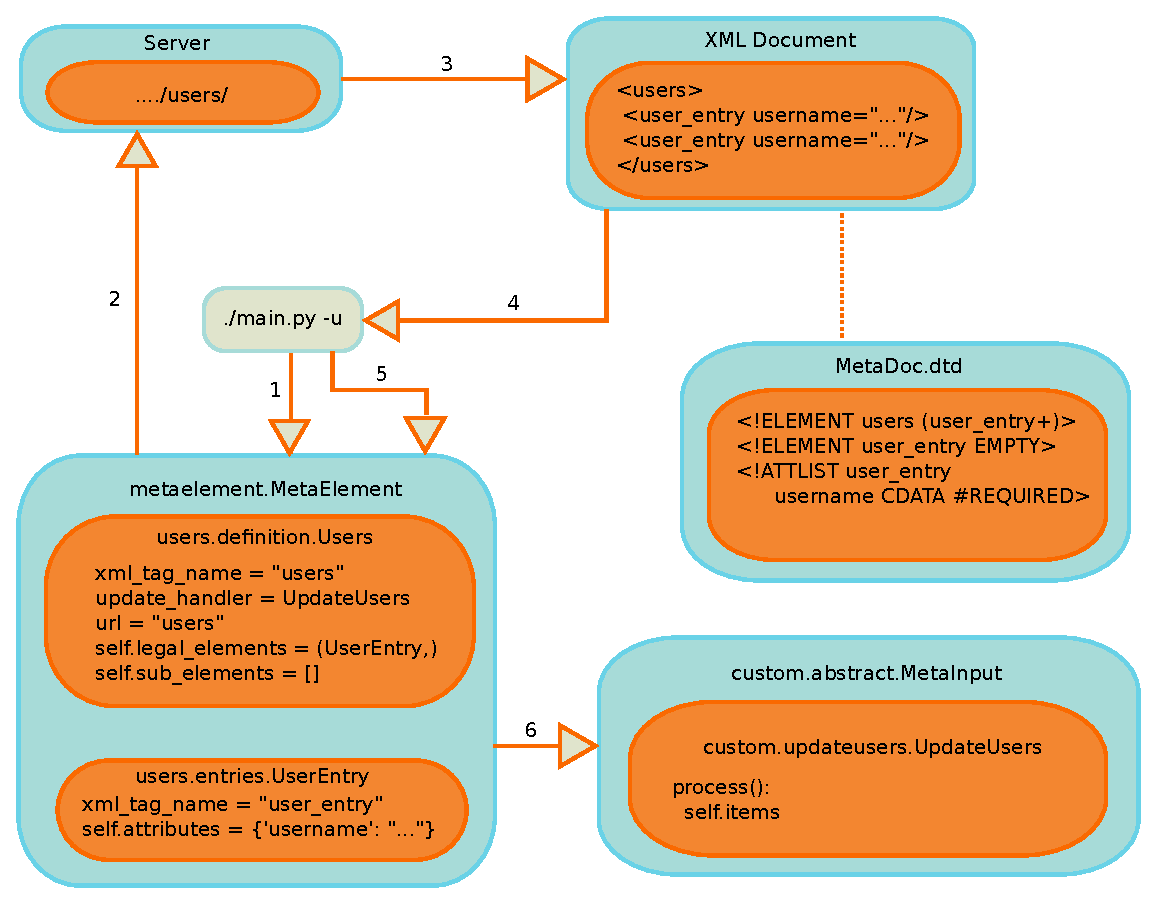
\includegraphics[width=\textwidth]{img/xml_flow}
    \caption{Information flow when requesting user list with MetaDoc}
    \label{fig:information_flow}
\end{figure}

Figure \ref{fig:information_flow} shows how information passes when a client
requests a user list. The steps are as follows:

\begin{enumerate}
    \item
        \texttt{main.py} is run with the handle \textbf{-u}, which will check
        \texttt{users.definition.Users} for which URL to access on the server
        to retrieve the information.
    \item
        A request is sent to the server to retrieve the information.
    \item
        The server creates an XML document with a list of users for the site.
        
        The XML document sent is defined by the MetaDoc DTD.
    \item
        \texttt{main.py} recieves the XML document, checks that it is valid
        according to the DTD. 
    \item
        If the XML document passes validation, an instance of
        \texttt{users.definition.Users} is created, and an instance of
        \texttt{users.entries.UserEntry} is created for each
        \texttt{<user\_entry>} in the XML document.

        \texttt{users.definition.Users} and \texttt{users.entries.UserEntry}
        may validate attributes and refuse to create any elements where
        attribute validation does not pass.
    \item
        The list of validated \texttt{users.entries.UserEntry} instances is
        placed within \texttt{self.items} for an
        \texttt{custom.updateusers.UpdateUsers} instance, and the
        \texttt{process()} function is called for the processing of the user
        list.
\end{enumerate}

\subsection{Validation}

\begin{figure}[h!]
    \includegraphics[width=\textwidth]{img/site_information_flow}
    \caption{Shows validation procedures when data is passed from client to
    server}
    \label{fig:site_information_flow}
\end{figure}

\begin{figure}[h!]
    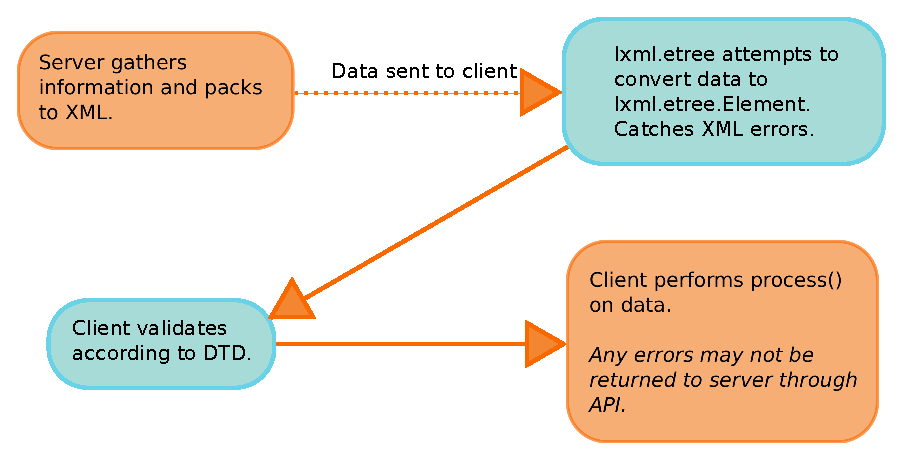
\includegraphics[width=\textwidth]{img/server_information_flow}
    \caption{Shows validation procedures when data is passed from server to
    client}
    \label{fig:server_information_flow}
\end{figure}


\newpage
\section{Errors}
\label{sec:errors}

The server returns a \texttt{<receipt>} containing an \texttt{<r\_entry>}
\textit{for each} element passed. The \texttt{<r\_entry>} has the required
attributes \textbf{id} and \textbf{code}, containing the ID of the element sent
by the client and the error code, respectively. It may also contain an
attribute \textbf{note} with a short note explaining the error if extra
information is available. The \texttt{<r\_entry>} tag might also contain text
with a longer message, if more information is needed about the error. 

An example of a error message would be an error code \texttt{2001} with the
note \texttt{Missing attribute "reason"}.

A list of possible return codes is given in table \ref{tbl:server_return_codes}
in appendix \ref{app:server_return_codes}. The difference between critical and
non-critical errors are that critical errors are problems with the element
itself, causing it to be refused by the server at any time. Non-critical errors
are errors where the element would potentially be accepted at a later date, but
not now.

\subsection{Document errors}

In the special case where there are problems with the document itself, such as
\gls{xml} errors or the document not passing \gls{dtd} verification, the
\texttt{<r\_entry>} \textbf{id} attribute will be set to \texttt{0} (zero),
referring to the document itself. 


\newpage
\begin{thebibliography}{99}
    \bibitem{improvingflow} Austad, Henrik, \textit{Improving the Information
    Flow within the Metacenter},
    \url{http://www.austad.us/metadoc/improvingFlow.pdf}
    \bibitem{quick_start_guide} Fjær, Bjørnar Grip, \textit{MetaDoc Quick Start
    Guide}, \url{http://bjornar.me/metadoc/quick_start_guide.pdf}
    \bibitem{metadoc_dtd} \textit{MetaDoc Document Type Definition}, 
        \url{http://bjornar.me/metadoc/MetaDoc.dtd}
    \bibitem{rfc3339} \textit{RFC3339}, \url{http://www.ietf.org/rfc/rfc3339.txt}
    \bibitem{python_modules} \textit{Python modules},
    \url{http://docs.python.org/tutorial/modules.html}
\end{thebibliography}


\appendix

\listoffigures

\listoftables

\lstlistoflistings

\printglossaries

\newpage
\section{List of errors}

\begin{table}[h]
    \caption{Error codes recieved from server}
    \begin{tabular}{|l|l|p{5cm}|}
        \hline
        \texttt{Error code} & \texttt{Meaning} & \texttt{Extra notes} \\
        \hline
        \hline
        1000 & No errors & \\
        \hline
        \hline
        2000 & Error with the XML data & \\
        \hline
        2001 & Missing attribute & Missing attribute should be returned as a note. \\
        \hline
        \hline
        5000 & Database error & \\
        \hline
        5001 & MySQL database error & Note should contain the MySQL error code, 
        and the message the MySQL error message \\
        \hline
        \hline
        6001 & Another element error & Another element in the same set has been
        rejected, and this type of set will not accept any elements if any
        element contains an error\\
        \hline
    \end{tabular}
    \label{tbl:server_error_codes}
\end{table}


\newpage
\section{Included examples}
\texttt{doc/examples/} includes a set of examples for using MetaDoc. Below is a
list of the included examples and what they do. 

\begin{description}
    \item[cli/event.py] A command line interface for adding events. Should be
    placed inside \texttt{client/} when run. See \texttt{event.py --help} for
    usage.
    \item[custom/updateusers.py]    Custom function for converting recieved
    user data into a passwd/shadow file.
    \item[custom/updateprojects.py] Custom function for converting recieved
    project data to a project user file.
    \item[custom/updateallocations.py]  Custom function for converting recieved
    allocation data into a quota file for projects.
    \item[configuration/metadoc.conf]   Example configuration file.
    \item[metaelements/]    Complete example of packages, modules and classes
    used to define a new type of data to send.
    \item[xml/] Examples of MetaDoc XML documents.
\end{description}


\end{document}
